%!TEX root = ../master.tex

\chapter{Implementation}\label{ch:implementation}
A lot of different methods exist to make this project possible. This chapter starts out with descriptions of the methods and theory behind the hardware and alternatives to the used methods. The chapter ends with descriptions of the used methods in the software. 


\section{Rear Diffused Illumination} \label{sec:RDI}
\begin{figure}[!h]
\centering	\includegraphics[width=0.5\textwidth]{sketchAugmentedBoard}
 \caption{A sketch of the RDI table.\label{Fig:sketch}}
\end{figure}
The interaction on the game board table is based on Rear Diffused Illumination as described in Multi-Touch Technologies \citep{multiTT}. This means, as shown in Figure \ref{Fig:sketch}, that infra-red (IR) lamps are placed underneath the table's surface, projecting IR light upwards. A webcam below the table is equipped with a visible light filter obtained from a floppy disc, meaning it primarily detects IR light. Furthermore, the table's surface, made of transparent material, needs a diffuser material just above or beneath it in order to diffuse the light. The purpose of this diffuser is to scatter the IR light and make objects hovering over the surface less visible to the camera. When an object touches the surface, the area of contact reflects more IR light than the untouched areas of the diffuser. This reflected light is captured by the camera, and can then be extracted as a BLOB. The diffuser has the additional purpose of facilitating a projection of the user interface from below.

\begin{figure}[!h]
\centering	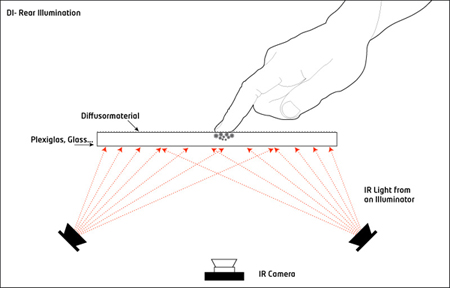
\includegraphics[width=0.5\textwidth]{RDItouch}
 \caption{Rear Diffused Illumination, illustrated by NUI Group \citep{multiTT}\label{Fig:RDI}}
\end{figure}

Choosing such a solution has its advantages and disadvantages. First of all, there is no need for a silicone rubber overlay, called a compliant surface, which normally would be needed for a FTIR solution \citep{multiTT}, as described in Section~\ref{technologiesAlternatives}. There is also no need for soldering an LED frame, since we are using a diffuser in order to reflect the IR light coming from below. The lamps for that can be bought ready to go, so there is no need to build them. A disadvantage comes from the RDI having difficulties with getting even illumination, since the IR lights might not cover the table's surface completely, or they might overlap, causing areas with an excessive amount of reflected IR light. This can result in false BLOBs, as well as BLOBs of lower contrast which are hard to detect. All this can challenge the software's detection of the desired BLOBs.

\subsection{Multi-Touch technology alternatives}\label{technologiesAlternatives}
Besides RDI, other solutions are presented in Multi-Touch Technologies \citep{multiTT}:

\textbf{Frustrated Total Internal Reflection (FTIR):} Instead of shining light from below, IR LEDs are projecting IR light directly into the acrylic glass from the side, which causes a total internal reflection. That means that until the user touches the surface, the IR light is totally reflected inside the glass. Once the surface is touched, the light rays are 'frustrated', causing the light to go downwards, which a webcam can capture in the same manner as with RDI. FTIR requires soldered IR LEDs, acrylic glass, a baffle to hide leaking LED light from sides of the glass, a diffuser, and a compliant layer which acts as a touch proxy, since it will improve the performance of FTIR.

This solution does not require an enclosed box, has strong contrasted BLOBs, allows varied BLOBs depending on touch pressure, and can, with a compliant surface, be used with even smaller tips than fingers have. Furthermore, it does not have the problem of uneven illumination which is present with RDI. However, it requires a soldered LED frame and a compliant surface, which makes it an impractical solution for this project.

\textbf{Front Diffused Illumination (FDI):} Visible light is shone from above the touch surface. This requires a glass surface with a diffuser layer. The camera captures the shadow created by contact with the surface. This solution requires no compliant surface, no LED frame, no soldering and no enclosed box, which makes it the simplest set-up of them all. It can make use of any transparent material and it can track fingers both touching and hovering, since both still creates the shadow needed.

The problem with this solution is that it cannot track objects. It also has difficulty avoiding false BLOBs and get even illumination, which makes it less reliable. This solution is not optimal when working on a digital board game, as the camera would catch too many shadows without players touching the board. This would cause problems, as players need to be able to gesticulate to each other during the game.

\textbf{Laser Light Plane:} This solution works by having a 1mm thick plane of IR light shined right above the surface by lasers. Whatever is in close contact with the surface, for example a fingertip, causes the light to scatter downwards to be captured by a webcam. Just as with FDI, LLP has a simple set-up which can use any transparent material as surface, and does not require an LED frame, an enclosed box or a compliant surface. It is also described as a cheap solution. The problems with LLP lies it its inability to track objects and being pressure sensitive. More importantly, it can have problems with the fact that several touches or objects can block the lasers for each other. This could be a problem, if we for example had game pieces on the board, which makes this solution unusable for this project. 
 
\textbf{Diffused Surface Illumination:} Almost as with the FTIR set-up, but without a compliant surface, the DSI solution makes use of Endlighten acrylic. This kind of acrylic redirects light evenly throughout the surface of the glass. Touches on the surface disrupts the light on contact, which creates contrasts that can be captured by a webcam. DSI is also pressure sensitive, due to the nature of how touch influences the light, and it can detect objects. Its disadvantages lie in the Endlighten acrylic's price, possible size restriction because of the special acrylic's softness, and a lower contrast than the FTIR and LLP. Especially the restrictions and lower contrast made this solution less favourable than the others.

\textbf{LED Light Plane:} With some similarities to FTIR and LLP, LED-LP has IR LEDs from the sides, but without an acrylic layer to move through, it is instead shone over the touch surface, which can be of any transparent material. A webcam captures the LED light cast on objects above the surface. This can require some patience with filter settings, since objects will light up due to the conical shape of the LED. The solution requires no enclosed box, which with the other requirements makes it a possibly cheap solution. It still needs an LED frame and very narrow-beamed LEDs, and it does not track objects while it still might purposelessly detect hovering due to insufficient filter settings. Since the solution is mentioned to be most suited for a LCD set-up and the hovering disadvantage might take up too much work, the solution is too impractical for the project.

\section{Physical Design} 
\begin{figure} [!h]
\centering 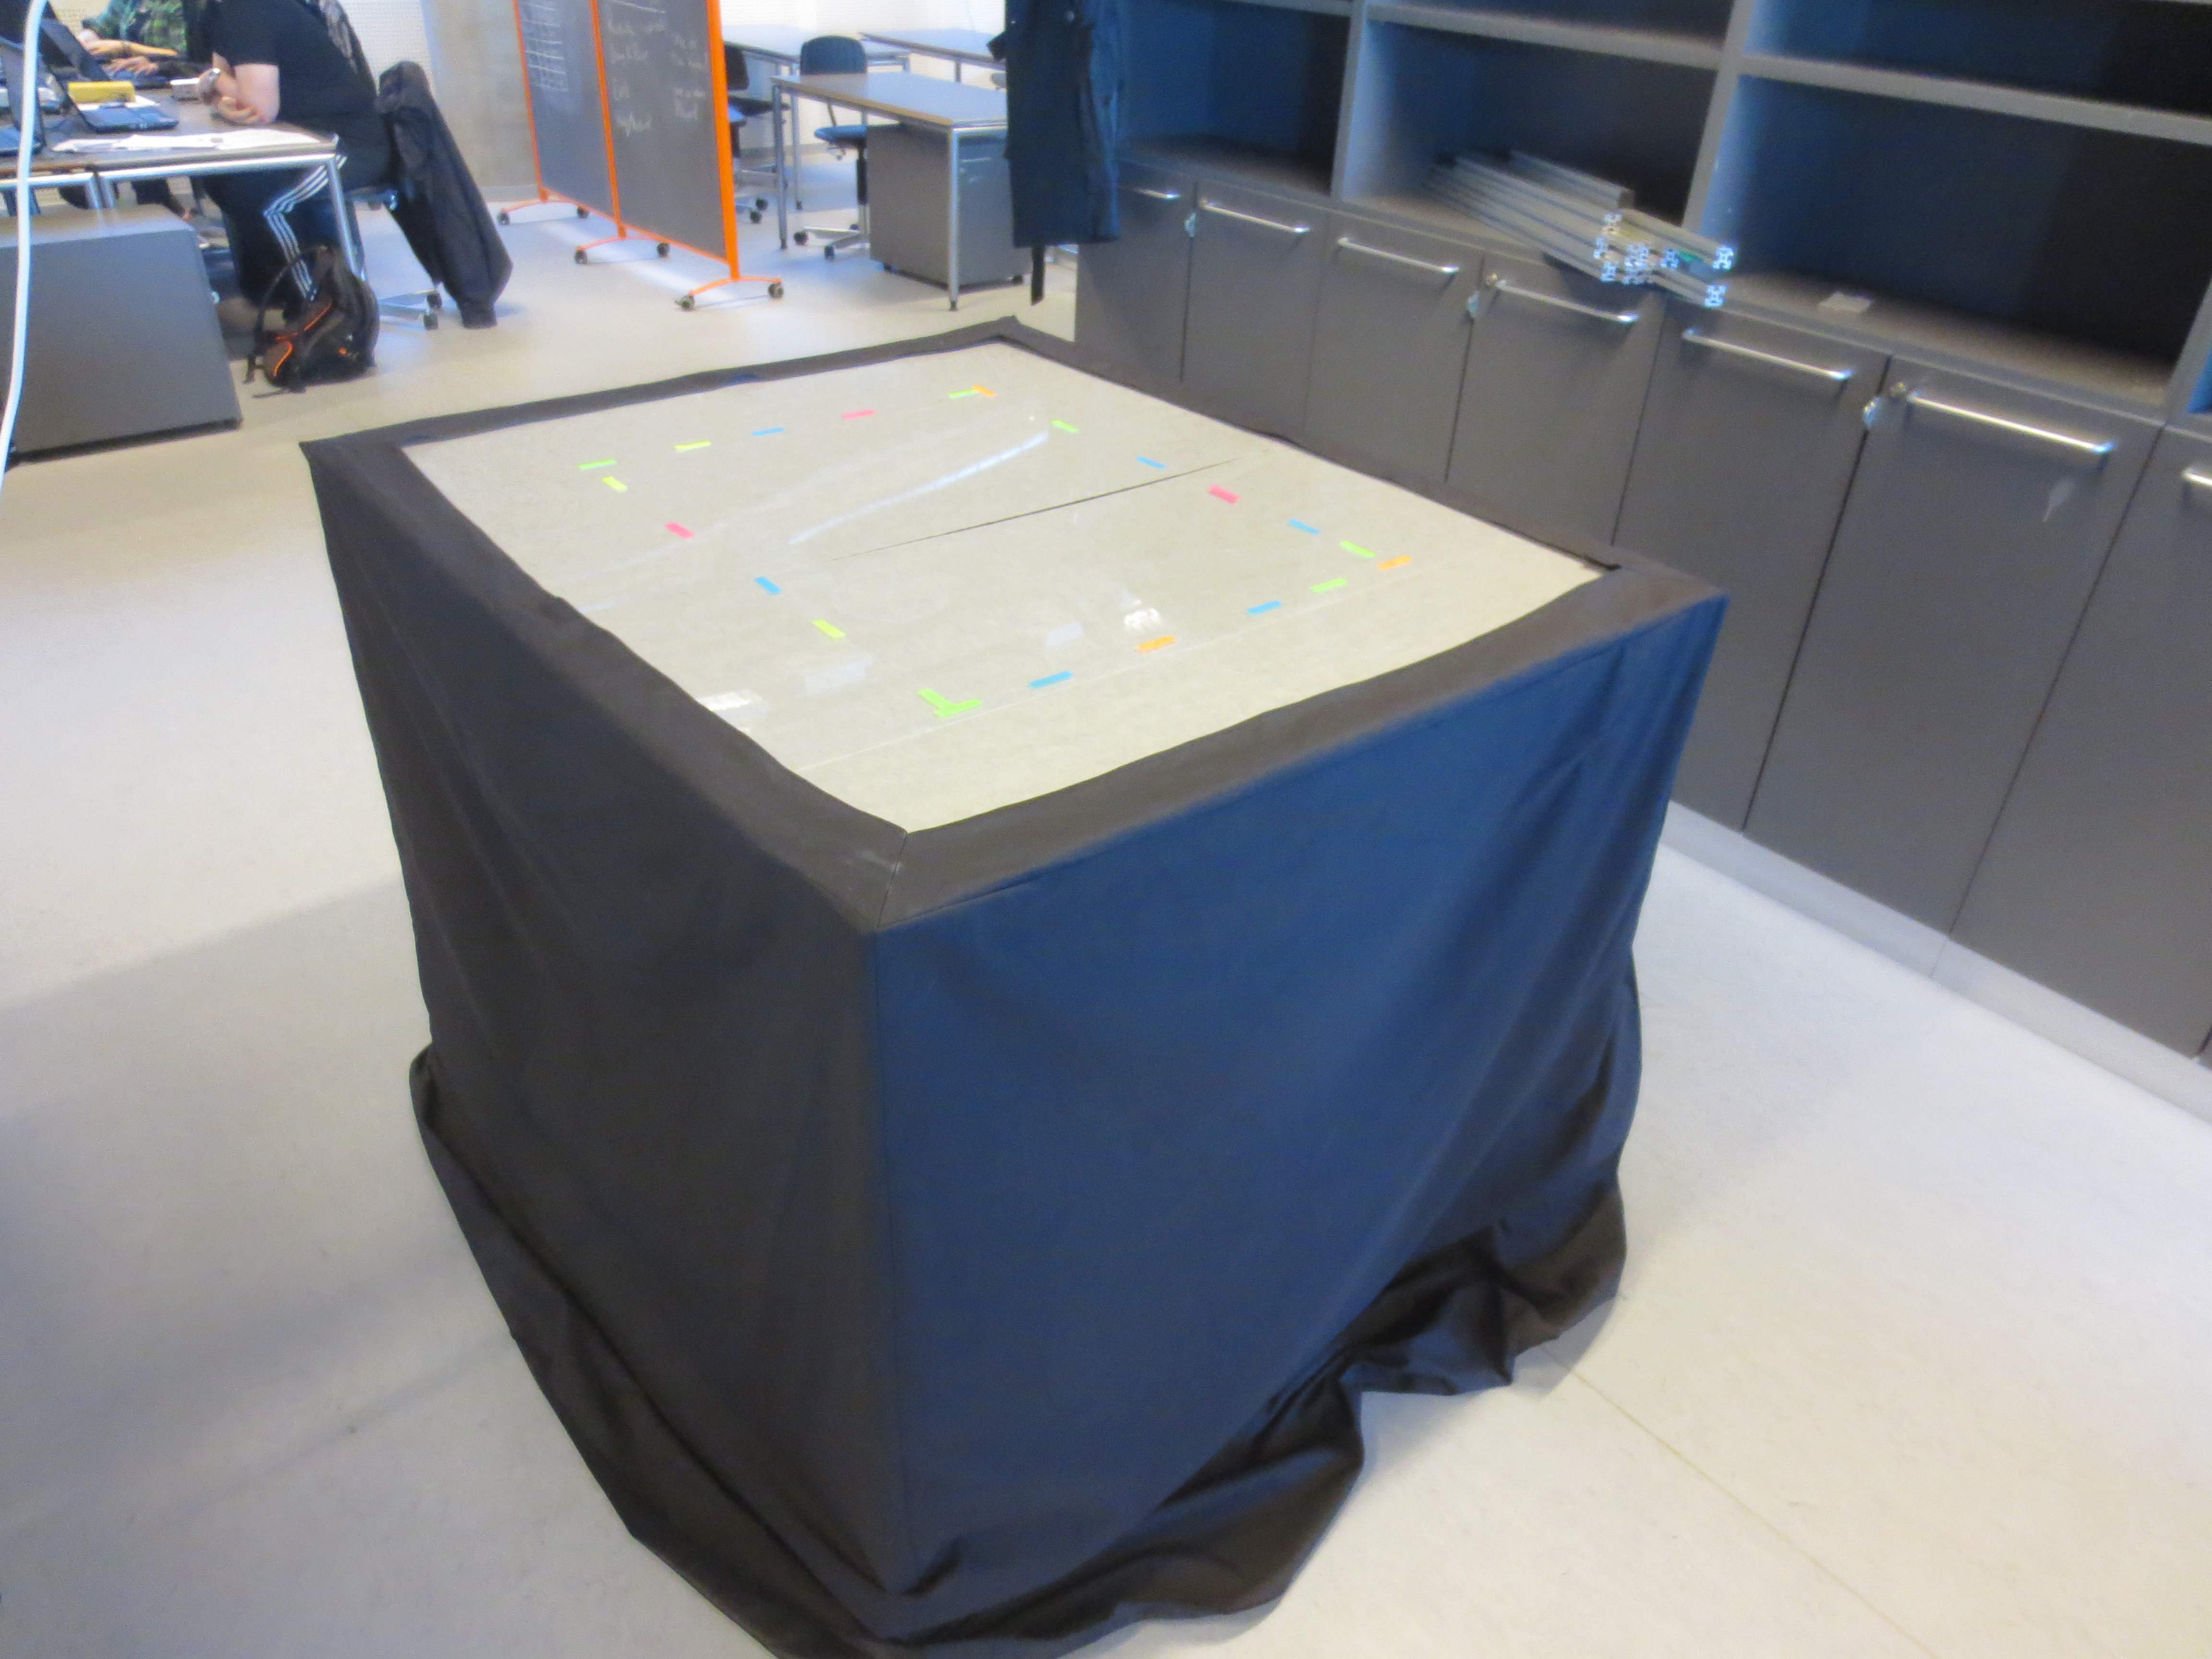
\includegraphics[width=0.5\textwidth]{Table}
 \caption{The touch table \label{Fig:Table}}
\end{figure}
This section will describe the physical aspect of the product.
The table's surface is made from acrylic glass, and below are four IR lamps, as well as a webcam with a visible light filter, and a short-throw projector, which will project images on the table. The webcam and IR lamps are there to facilitate RDI, as explained in Section~\ref{sec:RDI}. All these elements are placed in a manner that spreads the IR light from the lamps as evenly as possible.

The outer frame of the table is constructed from 3 different lengths of aluminium extrusions, giving the table a final size of 120 x 102 x 89 cm.
In order to keep outside IR light from disturbing the image as much as possible, black cloth covers the table at the sides as a baffle. The cloth has the additional benefit of making the projection from the short-throw projector clearer. 

As diffuser material, baking paper is used, as it is easily available. The paper is placed underneath the glass surface, as tightly as possible, as placing it on top results in too much light being reflected by the acrylic glass into the webcam. If the diffuser is not attached tightly enough to the glass, touching the surface does not result in enough IR light being reflected. The diffuser also works as a screen by blocking the light from the projector. 

\section{Image Processing}
To facilitate user interaction, a software module is needed to analyse a video input and recognize specific features and changes over time. As described in Section~\ref{sec:ReqSpec}, there are two main criteria for this software's minimum implementation. It needs to:
\begin{itemize}
\item Recognise which gesture is done when switching player.
\item Recognise when a tile is selected for terraforming.
\end{itemize}

To do these, BLOBs need to be extracted from the video input through segmentation.  

Furthermore, since this is a video feed rather than a static image, several of the methods in use will have to be looped. This leads to a two-step solution for processing the video input:

\begin{enumerate}
\item Segment image (Segmentation, includes de-noising/smoothing).
\item Conditionally change data depending on the BLOB analysis (Recognition and presentation)
\end{enumerate}


\subsection{Segmentation}
There are several methods for segmenting images. The relevant methods are discussed in this section. 

It is simpler, both from a computational and a programming standpoint, to process greyscale images as opposed to colour images. In this project, there is no benefit to using colour images as video input. Therefore, the video input is converted to greyscale. This is done by finding the mean of the RGB values in each pixel of the video input using the equation shown in Figure~\ref{fig:rgbToGreyEquation}.

\begin{figure}[h]
	\centering
	\begin{displaymath}
	I = \frac{R + G + B}{3}
	\end{displaymath}
	\caption{The returned intensity value I, is the mean of R, G, and B. \label{fig:rgbToGreyEquation}}
\end{figure}

As the project deals with video as opposed to static images, there is an issue with image noise. As the input from the camera is constantly updating, the noise is not static. Therefore, a smoothing filter is necessary, so more noise can be negated. In this case, a Gaussian blur is implemented.

\begin{figure}[h]
  \begin{center}
    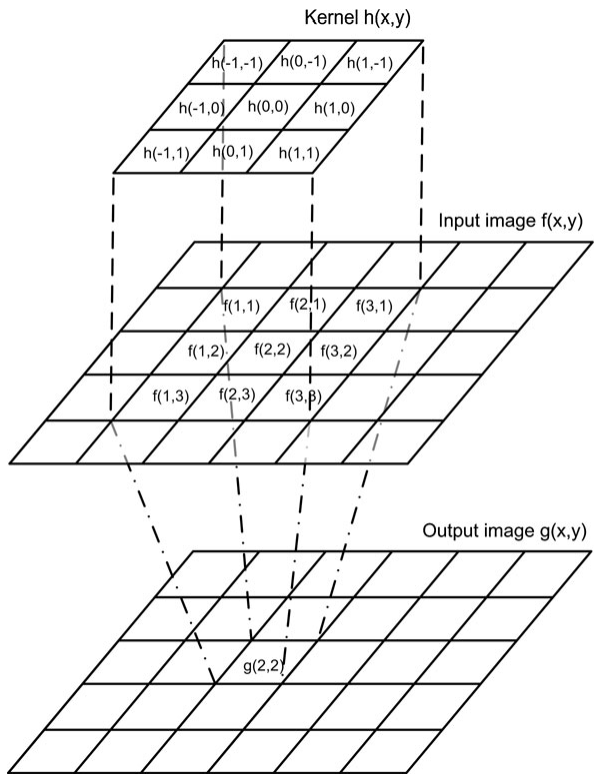
\includegraphics[width=0.5\textwidth]{Correlation}
  \end{center}
  \caption{A visualisation of correlation \label{Fig:Correlation}\citep{moeslund_introduction_2012}}
\end{figure}

A Gaussian blur is a correlation-based image processing operation, which makes use of a kernel. This works by imposing the kernel on top of the pixels of the image that is processed, as illustrated in Figure~\ref{Fig:Correlation}. The pixel that will be processed for each placement of the kernel is the one that corresponds to the middle pixel of the kernel. This means that the border of the image will be lost when doing this operation, as the kernel cannot be applied to the outermost pixels without going out of bounds. The new pixel value is calculated by multiplying each value in the kernel with the value of its corresponding pixel and finding the sum of these values using the equation shown in Figure~\ref{fig:gaussianEquation}, where g(x, y) returns the value of the output pixel, R is the radius of the kernel, and f(x, y) is the input pixel \citep{moeslund_introduction_2012}. Each of these results are then divided with the sum of the kernels' coefficients to normalise the output image. The resulting number is the new value of the pixel being processed.

\begin{figure}[!h]
	\centering
	\begin{displaymath}
	g(x,y) = \sum^R_{j=-R} \sum^R_{i=-R} h(i, j) \cdot f(x + i, y + j)
	\end{displaymath}
	\caption{Equation for applying a gaussian kernel to an image. \label{fig:gaussianEquation}}
\end{figure}

The Gaussian kernel, displayed in Figure \ref{Fig:Gaussian}, is a kernel with a specific pattern. This pattern gives more weight to the pixels paired with the centring kernel values, thereby giving them more influence in the image processing. It is used to remove detail from an image, which as mentioned earlier is useful to remove noise.

\begin{figure}[h]
\begin{center}
 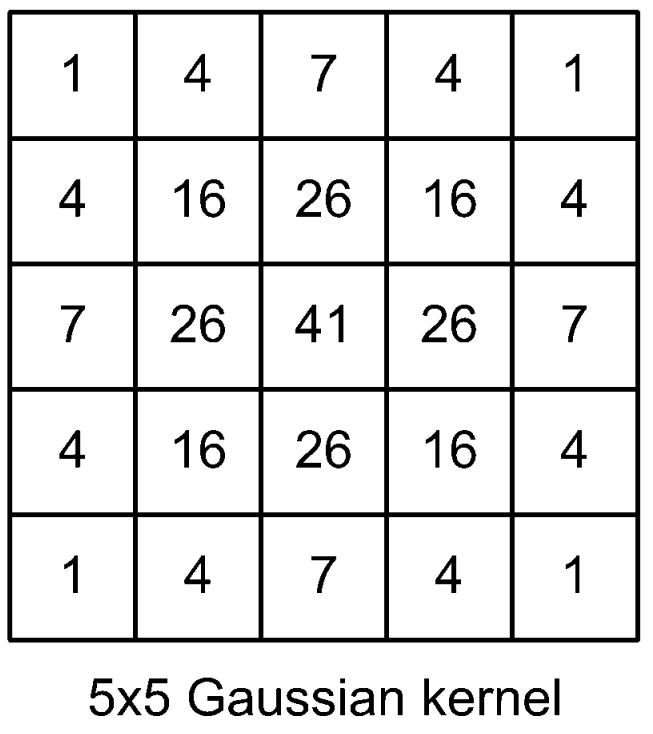
\includegraphics[width=0.3\textwidth]{Gaussian}
  \end{center}
\caption{A 5x5 Gaussian kernel pattern \label{Fig:Gaussian}\citep{moeslund_introduction_2012}.}
\end{figure}

In order to create a binary image containing BLOBs, the images of the video need to be thresholded. In an ideal image which is to be thresholded, the histogram will have two distinct 'mountains' of pixel values, that is to say, there will be two groups of pixels with similar brightness. Ideally, the groups are isolated from each other in brightness. Achieving such an image is the purpose of the processes that have been described so far. In the case of this project, the image produced is expected to have bright spots where the board is touched, on a dark plane which is to be considered the background.

Once this type of image is achieved, it can be thresholded. The program aims to make every pixel that should be considered relevant input white, and to make every other pixel black, which is considered the background. As described in Section~\ref{sec:RDI}, the hardware setup uses RDI with IR light sources, and a visible light filter on a web camera, meaning that contact with the surface should create BLOBs. The image is made binary by choosing a reasonable threshold representing a certain pixel value, and then for each pixel determining whether its value is above or below this value. If it is equal to or above the given value, the pixel becomes white. If it is below the given value, it becomes black.
 
\subsection{Morphology}
After thresholding the image, small unwanted spots of white pixels appear on the background where no input is given. In order to negate this, the \textit{opening} process is applied. This consists of two operations: an \textit{erosion} operation followed by a \textit{dilation} operation \citep{moeslund_introduction_2012}. The erosion operation removes the majority of the white noise on the background, but the large BLOBs that are meant to be detected are also reduced in size. This is when the dilation operation is called, which dilates the already eroded BLOBs. This affects the BLOBs large enough to not be removed by the erosion, but the noise will not be dilated, as they are removed during the erosion operation.

\begin{figure}[!h]
	\centering
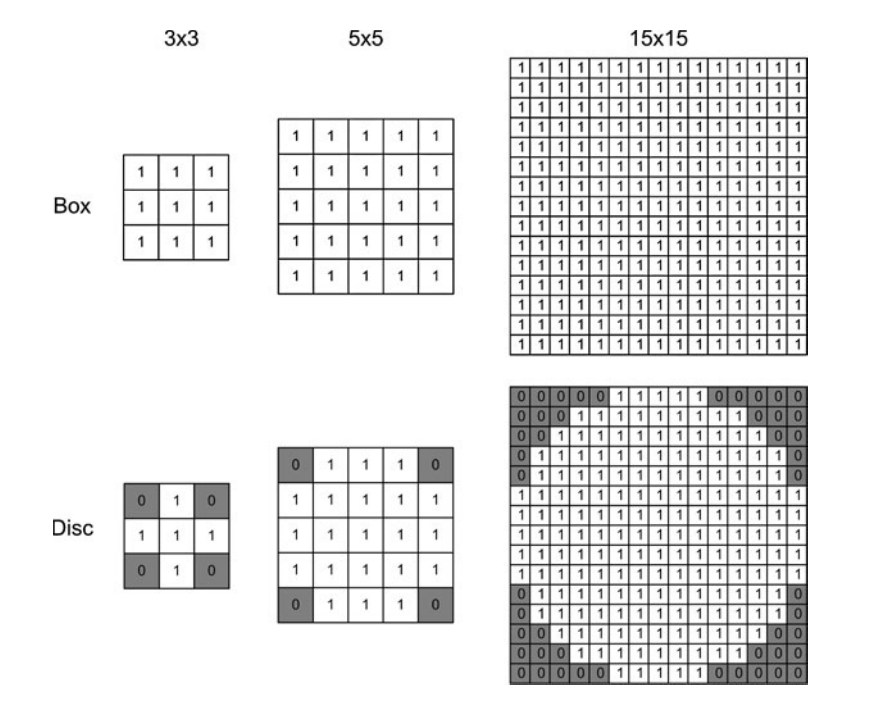
\includegraphics[width=0.7\textwidth]{StructuringElements}
\caption{Two types of structuring elements of different sizes \citep{moeslund_introduction_2012}. \label{fig:StructuringElements}}
\end{figure}

\begin{figure}[!h]
	\centering
	\begin{displaymath}
	g(x, y) = f(x, y) \oplus SE
	\end{displaymath}
	\caption{Mathematical equation for dilation \citep{moeslund_introduction_2012}. \label{fig:dilateEquation}}
\end{figure}

\begin{figure}[!h]
	\centering
	\begin{displaymath}
	g(x, y) = f(x, y) \ominus SE
	\end{displaymath}
	\caption{Mathematical equation for erosion \citep{moeslund_introduction_2012}. \label{fig:erodeEquation}}
\end{figure}

These morphology algorithms work by applying a \textit{hit} or \textit{fit} operation to each pixel making use of a structuring element. The most common types of structuring elements are \textit{box} and \textit{disc} shaped. Examples of these can be found in Figure~\ref{fig:StructuringElements}. These strucuring elements are applied to an image using the appropriate mathematical function. For dilation, the equation shown in Figure~\ref{fig:dilateEquation} is used. For erosion, the equation shown in Figure~\ref{fig:erodeEquation} is used. In the \textit{opening} process, the operations are combined using the equation shown in Figure~\ref{fig:openingEquation}.

\begin{figure}[!h]
	\centering
	\begin{displaymath}
	g(x, y) = (f(x, y) \ominus SE) \oplus SE
	\end{displaymath}
	\caption{Opening operation \citep{moeslund_introduction_2012}. \label{fig:openingEquation}}
\end{figure}

\subsection{BLOB analysis}

The BLOBs created by user input need to be differentiated from any noise that may remain even after opening. To do this, each BLOB is given a convex hull. The convex hull of a BLOB is, as described by Moeslund, "\textit{... the minimum convex polygon which contains the BLOB. It corresponds to placing a rubber band around the BLOB.}" \citep{moeslund_introduction_2012} In this project, the area of a convex hull are calculated using Sklansky's algorithm \citep{Sklansky198279}. By filtering the convex hulls by size, while ignoring those that have a small area, a BLOB from a specific gesture can be detected.
\begin{figure}[h!]
\begin{center}
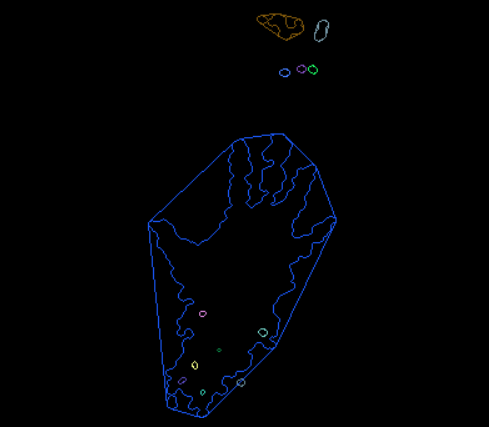
\includegraphics[width=0.5\textwidth]{Convex}
\end{center}
\caption{The convex hull of a hand \label{Fig:Convex}}
\end{figure}

\section{Rendering of game board}
In order for the program to be able to change the game tiles through terraforming, it must have access to them from the start. This is done by having the program render all the tiles. The border around the actual tiles are made from a background image, which is imported as is. This image contains the outline of a player area for each player, the point counter, and the icons for the global action. All this is illustrated in Figure~\ref{Fig:Board}.

\begin{figure}[!h]
\centering 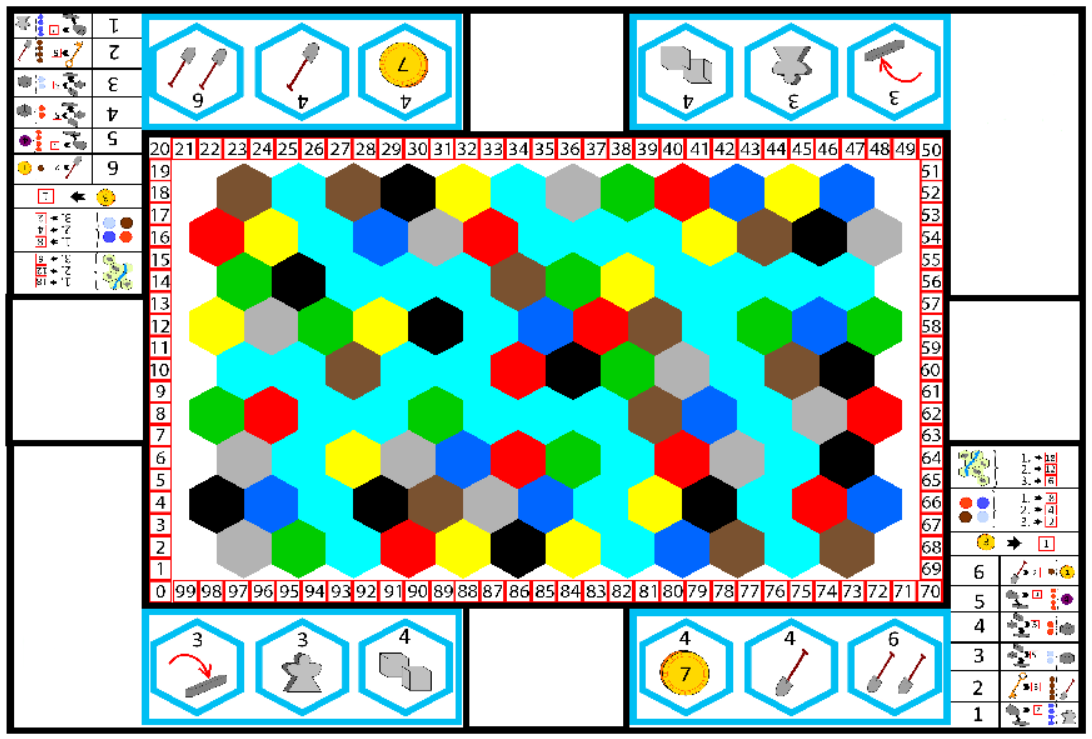
\includegraphics[width=0.5\textwidth]{BoardWithTilesNoUndo}
\caption{The game board \label{Fig:Board}}
\end{figure}

On top of this image, the tiles are rendered. This is done with a function, which takes a two-dimensional coordinate, the height of the hexagon, the image on which to draw, and a colour as parameters. The function calculates the radius based on the height input, which is then used to calculate the remaining points using the aforementioned parameters. Then the function fills it with the given colour. The equations used to calculate the points in the hexagon are shown in Figure \ref{Fig:HexWithMath}.

\begin{figure}[!h]
\centering 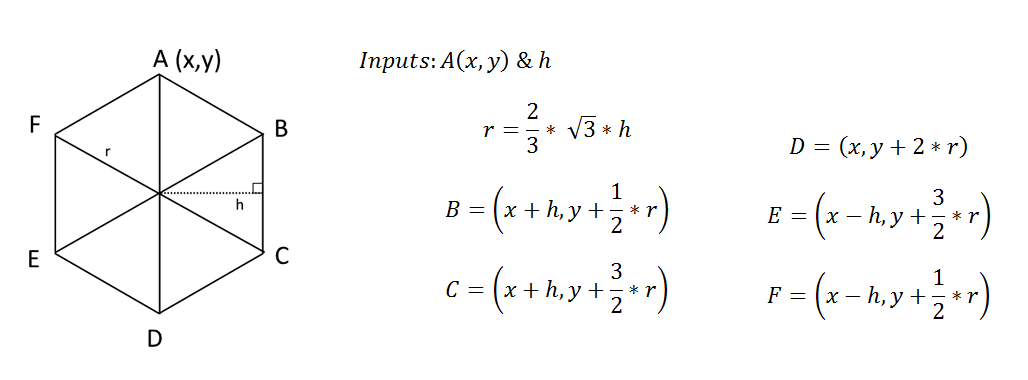
\includegraphics[width=0.8\textwidth]{HexWithMathv2}
\caption{Relations between height and points in hexagon \label{Fig:HexWithMath}}
\end{figure}

With this method, the program renders the board row by row, saving the coordinate of the A-point of each tile and the colour in two different arrays.